
\section{TJ-Monopix1 characterization}
    \subsection{Front end parameters}


    \subsection{Threshold and noise: figure of merit for pixel detectors}
        %python3 -i calibration/scurve_tot_histo.py -f calibration/calibration_data/20220506 -i 1 100 questo script crea i file di output contenenti i gli istogrammi del tot e della s curve
        %python3 -i calibration/tot_charge_plotting.py -f calibration/calibration_data/20220506 per fare il plot della s curve e relativi residui 
        %python3 -i calibration/tot_histo2d.py -f calibration/calibration_data/PMOS/20220506 per fare l'istogramma 2d del tot
        \red{Una caratterizzazione di soglia e rumore è necessaria in quanto questi valori condizionano sia le condizioni di operatività di questi chip, che le performance. }
        Infact, the signal to threshold ratio may be considered as the figure of merit for pixel detectors rather than the signal to noise ratio.
        The threshold has to be low enough to mantain a high signal efficiency, but also high enough to cut the noise: for a low threshold many pixels can fire at the same time and a positive feedback can set off a chain reaction eventually, causing all the other pixels to fire. 
        \red{Thus, the noise sets a lower bound to the threshold: if an occupancy $\leqslant$ $10^{-4}$ is required, for example, this correspond to the Gaussian 1-sided tail fraction for \SI{3.7}{\sigma}.
        In this case, if the noise is \SI{100}{e-}, for example, the threshold must be higher than \SI[parse-numbers=false]{3.7\times100}{e-}.}
        Typically this argument sets only a minimal bound to the threshold since the variation with time and from pixel to pixel have to be taken into account: the temperature, the anealing (for example, the radiation damages in the oxide layer causes shift of MOSFET threshold voltage) and the process parameters variation across the wafer (as for example process mismatch between transistors). 
        A requirement for the FE noise (the ENC is the equivalent input charge noise) is: 
        \begin{equation}
            ENC < \sqrt{(T/3.7)^2 - T_{RMS} ^2 (x) - T_{RMS} ^2 (t)}
        \end{equation}
        where the T is the threshold set, $T_{RMS}$ is the threshold variation during time (t) and across the matrix (x).

        For this reason is desiderable the possibility of changing and adapting the setting parameters of the FE, both in time and in space: this parameters are usually set by Digital to Analog Converter (DAC) with a number of bit in a typical range of 3-7.

        DAC elements require a lot of space that may be not enough on the pixel area. Therefore, the FE parameters are typically global, which means that they are assigned for the whole chip, or they can be assigned for regions the matrix is divided into. 
        The former case corresponds to TJ-Monopix1's design in which 7 bits are used for a total 127-DAC possible values, while the latter corresponds to the ARCADIA-MD1's one, \red{where quanti bit??}. 
        An other possibility, for example implemented in TJ-Monopix2, is allocate the space on each pixel for a subset of bits, then combinig the global threshold with a fine tuning. 

        To measure the threshold and noise of pixels a possible way is a scan with different known injected charge at a fixed threshold, that corresponds to the value where the efficiency of the signal exceeds the 50\%.
        Therefore, for a fixed threshold (I set IDB = 40 DAC to perform the scan) I have used the injection circuit available on the chip to inject 100 pulses for each input charge. 
        The injection comes on a capacity at the input of the FE circuit, whose mean value is \SI{230}{aF} (in section \ref{sec:} I'll present the calibration of the signal from which I also found the value of this capacity across the matrix). 
        For the PMOS flavors: since the DAC are biased at \SI{1.8}{V}, the Least significant Bit (LSB) corresponds to a voltage of \SI{14.7}{mV} from which the charge for LSB \SI{1.43}{e-/mV} and the conversion factor from DAC to electrons \SI{20.3}{e-/DAC} are obtained. 
        While this value is equivalent for all the PMOS flavor, the HV flavor is expected to have a different conversion factor, $\sim$ \SI{33}{e-/DAC}, beacuse of the different input capacity. 
        Besides the charge, also the duration and the period of the injection pulse can be set; it is important to make the duration short enough to have the falling edge during thed dead time of the pixel (in particular during the FREEZE signal) in order to avoid the undershoot, coming at high input charge, triggering the readout and reading spurious hits. 
        Since the injection circuit is coupled in AC to the FE, if the falling edge of the pulse is sharp enought to produce ad undershoot, this can be seen as a signal. 

        Assuming a gaussian noise, it can be described through the error function; actually, since the error function has y bounded between -1 and +1, the function I need is a modification of the $erf$: 
        
        \begin{equation}
            f(x, \mu, \sigma) = \frac{1}{2} \; \left(1\,+\,erf\left(\frac{x-\mu}{\sigma \sqrt{2}}\right)\right)
        \end{equation}
        \begin{equation}
            erf(z) = \frac{2}{\sqrt{\pi}} e^{-x^2} dx 
        \end{equation}   
            
    
        \begin{figure}[h!]
            \centering
            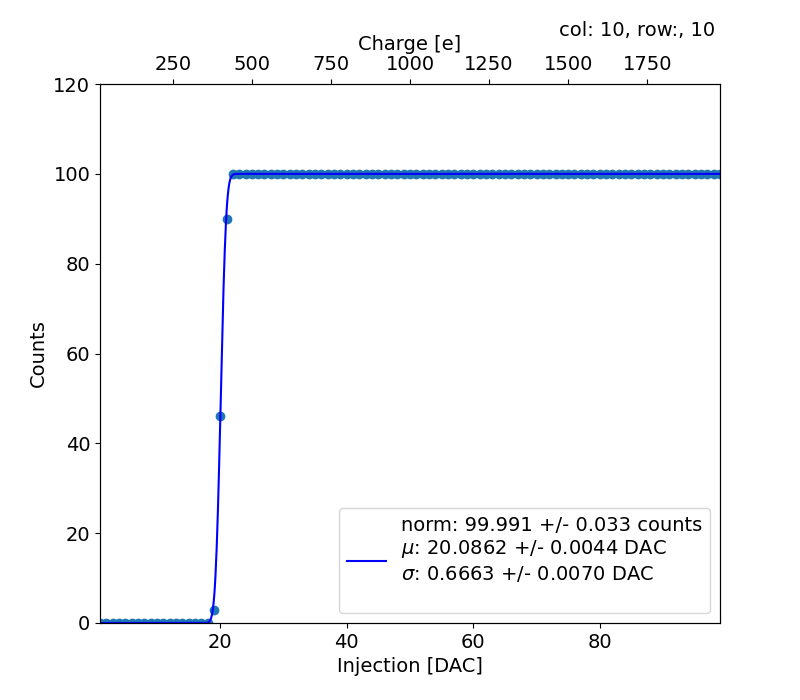
\includegraphics[width=.6\linewidth]{figures/charaterization/scurve.png}
            \caption{S curve for pixel (10, 10) of the PMOS flavor. The conversion of charge injected from DAC to electrons has been done assuming a conversion factor of \SI{20}{e-/DAC}.}
            \label{fig:scurve}
        \end{figure}   
        The mean minimum stable threshold evolved through different generation of chips: in the 1st generation it was around \SI{2500}{e-} while in the 3rd (corresponding to nowadays chips) is less than \SI{500}{e-}. This allows in thinner sensors with smaller signals: from \SI{16000}{e-} produced in \SI{200}{\um}, the signal expected moved down to \SI{2000}{e-} produced in \SI{25}{\um}. According with this \red{??}, the threshold of TJ-Monopix1 is around \SI{500}{e-}.
        \red{I successivi prototipi hanno una soglia e un rumore più bassi, ad esempio TJ-Monopix2 ha una soglia e un rumore... }
        The values of the threshold and the noise for the flavor are reported in tables \ref{tab:}
    
        \begin{figure}[h!]
                -\begin{subfigure}{.5\textwidth}
                \centering
                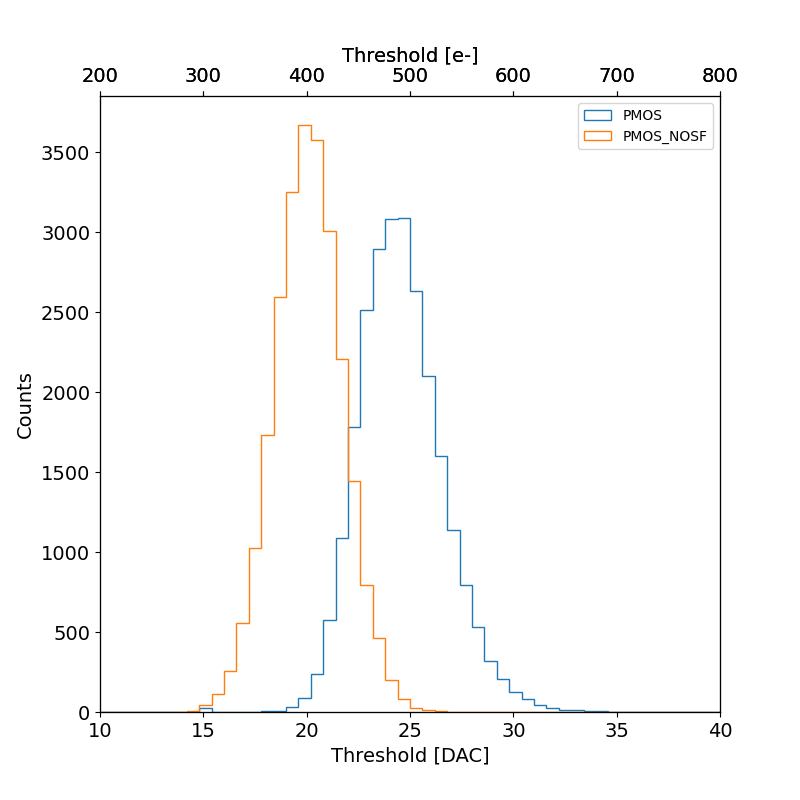
\includegraphics[width=.99\linewidth]{figures/charaterization/threshold_histogram.png}
                \caption{}
                \label{fig:}
                \end{subfigure}
                \begin{subfigure}{.5\textwidth}
                \centering
                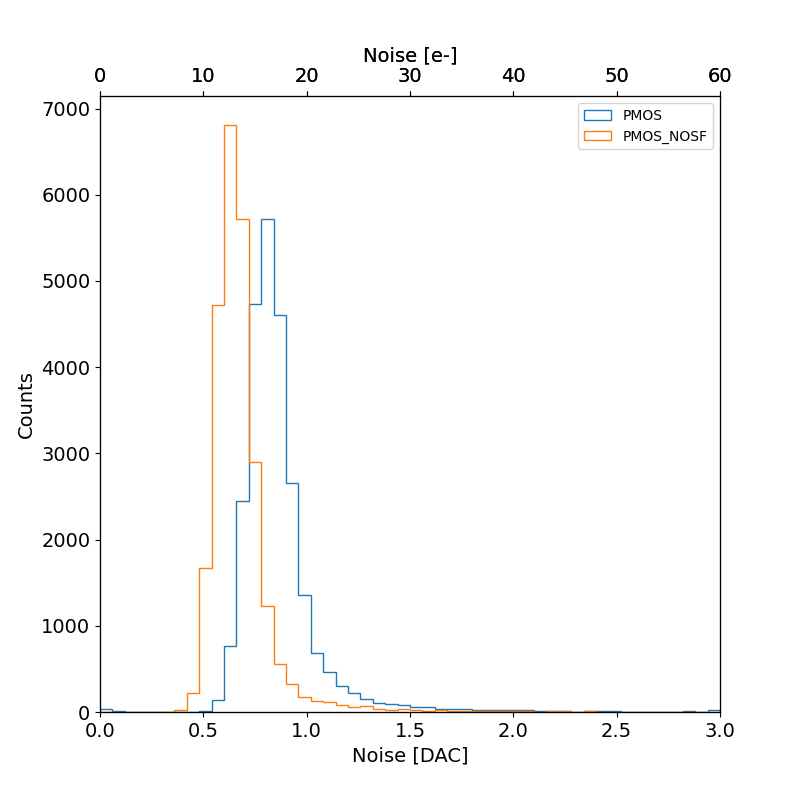
\includegraphics[width=.99\linewidth]{figures/charaterization/noise_histogram.png}
                \caption{}
                \label{fig:}
                \end{subfigure}
        \end{figure}            
           
        \begin{figure}[h!]
            \begin{subfigure}{.5\textwidth}
            \centering
            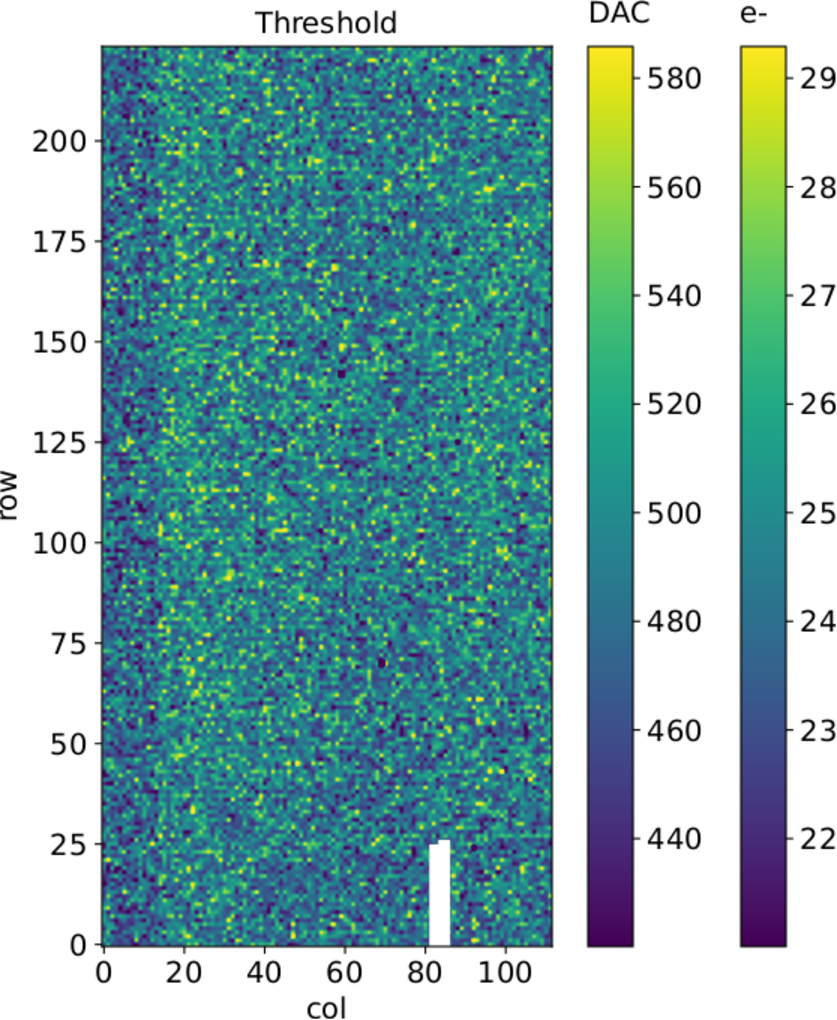
\includegraphics[width=.99\linewidth]{figures/charaterization/threshold_map.pdf}
            \label{fig:}
            \end{subfigure}
            \begin{subfigure}{.5\textwidth}
            \centering
            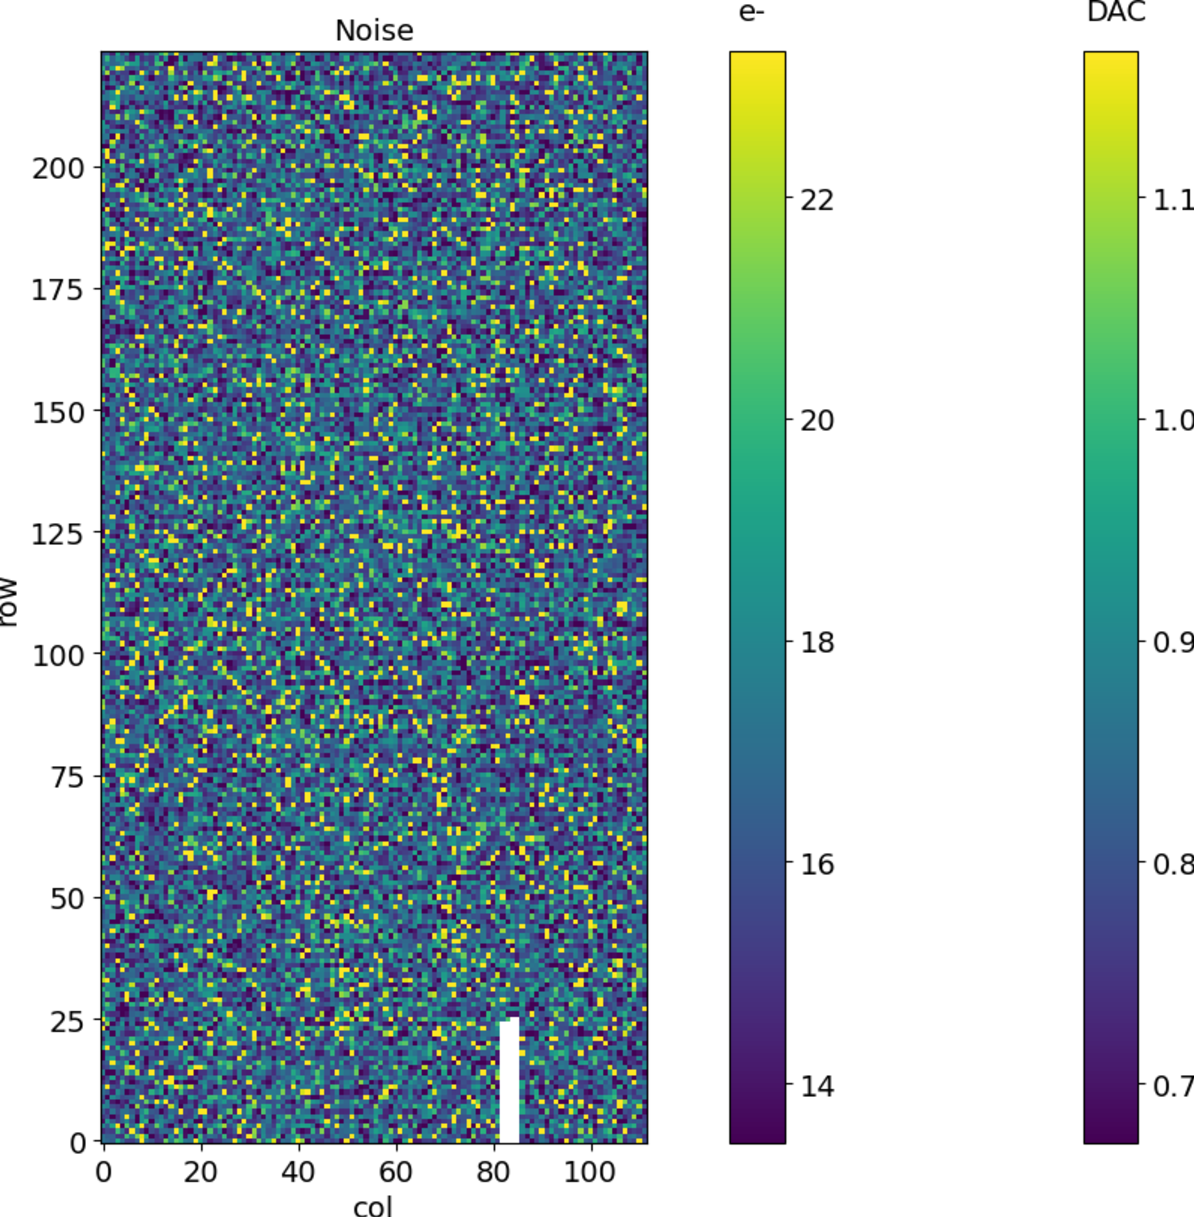
\includegraphics[width=.99\linewidth]{figures/charaterization/noise_map.pdf}
            \label{fig:}
            \end{subfigure}
            \caption{}
        \end{figure} 
    
        \begin{table}
                \begin{center}
                \begin{tabular}{| c | c | c |}
                \hline
                 & DAC units & electrons \\
                \hline
                \hline
                Threshold        & 24.529 $\pm$ 0.049 & \\
                                 &u: 24.433 $\pm$ 0.049 & \\ 
                                 &d: 24.623 $\pm$ 0.051 &    \\      
                Threshold dispersion & 1.848 $\pm$ 0.033 &\\
                                 &u: 1.867 $\pm$ 0.034 & \\ 
                                 &d: 1.825 $\pm$ 0.035 &    \\ 
                Noise            & 0.8222 $\pm$ 0.0043 & \\
                                 &u: 0.8225 $\pm$ 0.0045 & \\ 
                                 &d: 0.8221 $\pm$ 0.0043 &    \\      
                Noise dispersion & 0.0975 $\pm$ 0.0030 &\\
                                 &u: 0.0968 $\pm$ 0.0031 & \\ 
                                 &d: 0.0970 $\pm$ 0.0030 &    \\ 
                \hline
                \end{tabular}
                \caption{Flavor PMOS}
                \label{tab:}
                \end{center}
        \end{table}        
    
    \begin{itemize}
        \item disperione della soglia dovuta al DAC e confronta con il valore misurato
        \item dipendenza della soglia da IDB
        \item dipendenza della soglia dal gain
    \end{itemize}    
    La dispersione della soglia dopo al tuning e dovuta al dac è: 
        \begin{equation}
            \sigma_{THR, tuned} = \frac{\sigma_{THR}}{2^{n bit}}
        \end{equation}
    
        I also have perfmorm a scan for different IDB value to verified the trend of the threshold. 
    \red{MEtti plot della media della gaussiana in funzione di IDB}

    Dipendenza dal guadagno: per valutare l'impatto del discriminarore sul rumore uno dovrebbe convertire il segnale in uscita in segnale in carica all'ingresso. In questo modo si avrebbe:
    \begin{multicols}{2}
        \begin{equation}
            ENC_{DISC} = \frac{V_{noise} ^ {RMS}}{G}
        \end{equation}\break
        \begin{equation}
            ENC_{DISC} = \frac{V_{mis} ^ {RMS}}{G}
        \end{equation}
        \label{eq:}
    \end{multicols}
    where $V_{noise} ^ {RMS}$ is the RMS noise and $V_{mis} ^ {RMS}$ is the mismatch voltage at the discriminator input and G is the gain of the preamplifier. 
    Quindi, as the gain is increased, the discriminator influence in niise an threshold mismatch performance is reduced. Although the discriminator noise is relatively low compared to the preamplifier noise and can be neglected, the contribution to threshold dispersion can be significant due
    to the threshold variation of transistor M11

        

    \subsection{Calibration of the ToT}    
        %python3 -i acquisition_Fe55/fit_tot_single_pixel.py -f acquisition_Fe55/source_PMOSS/ per fare il fit    
        %python3 -i acquisition_Fe55/plot_tot_single_pixel.py -f acquisition_Fe55/source_PMOSS/ -fl 'gauss_line' per fare il plot di single pixel
        I have already said in chapter \ref{chap:} that TJ-Monopix1 returns an output signal propo 


        Abbiamo già detto che Monopix uno fornisce una misura della carica rilasciata dalla particella incidente attraverso il Time over Threshold of a triangular pulse e che il ToT viene salvato come variabile a 6 bit (da cui un range 0-64 escluso) con clock a \SI{40}{MHz}, per cui per un bit si hanno \SI{25}{ns}. 
        Per poter associare questo tempo ad una carica è necessaria una calibrazione del segnale: utilizzando l'iniezione è possibile studiare l'andamento del ToT con la carica iniettata. 
        Poichè, come già detto, l'impulso di iniezione dipende dalla C di iniezione, che sarà diversa per ogni pixel, per effettuare una corrispondenza tra tot ad elettroni è necessaria una calibrazione assoluta di questa capacità.

        \begin{figure}[h!]
            \begin{subfigure}{.5\textwidth}
            \centering
            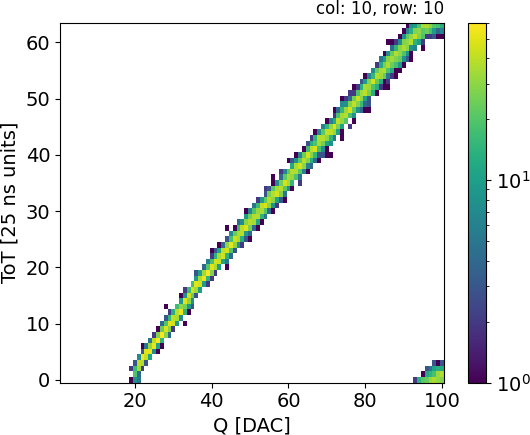
\includegraphics[width=.98\linewidth]{figures/charaterization/ToT_rollover.png}
            \label{fig:}
            \end{subfigure}
            \begin{subfigure}{.5\textwidth}
            \centering
            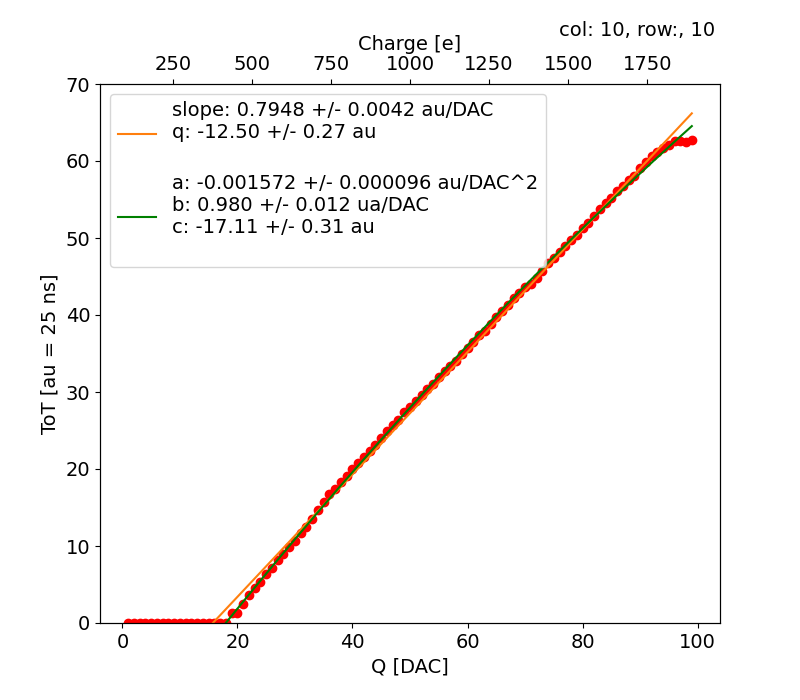
\includegraphics[width=.98\linewidth]{figures/charaterization/ToT_injection.png}
            \label{fig:}
            \end{subfigure}
            \caption{(a) ToT rollover for pixel (10,10). The ToT is in range 0-64 since it is represented by 6 bit; (b)}
        \end{figure}    

        \begin{figure}[h!]
            \begin{subfigure}{.5\textwidth}
            \centering
            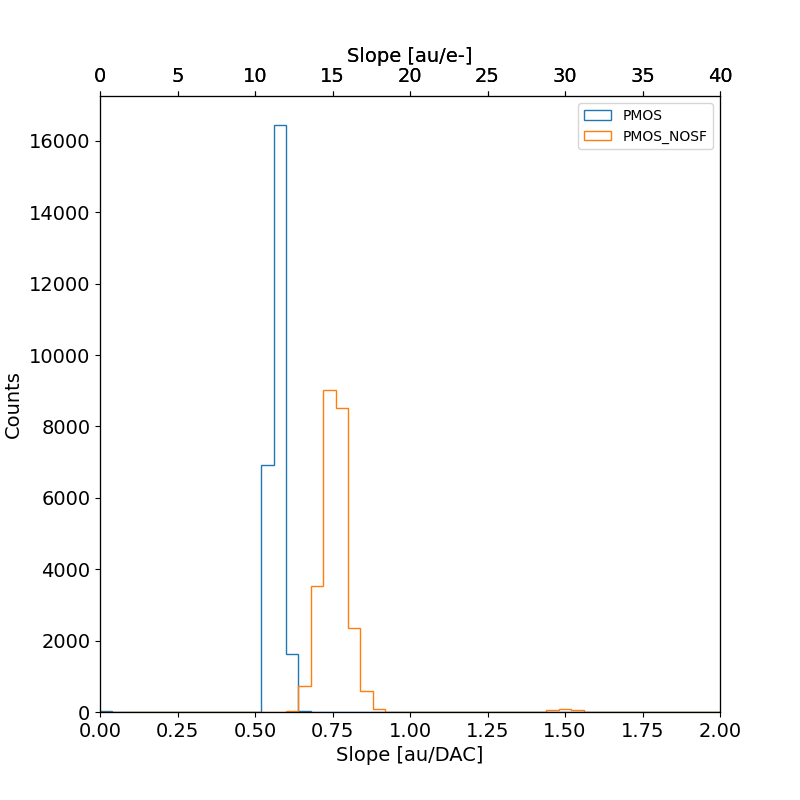
\includegraphics[width=.98\linewidth]{figures/charaterization/slope_histogram.png}
            \caption{}
            \label{fig:}
            \end{subfigure}
            \begin{subfigure}{.5\textwidth}
            \centering
            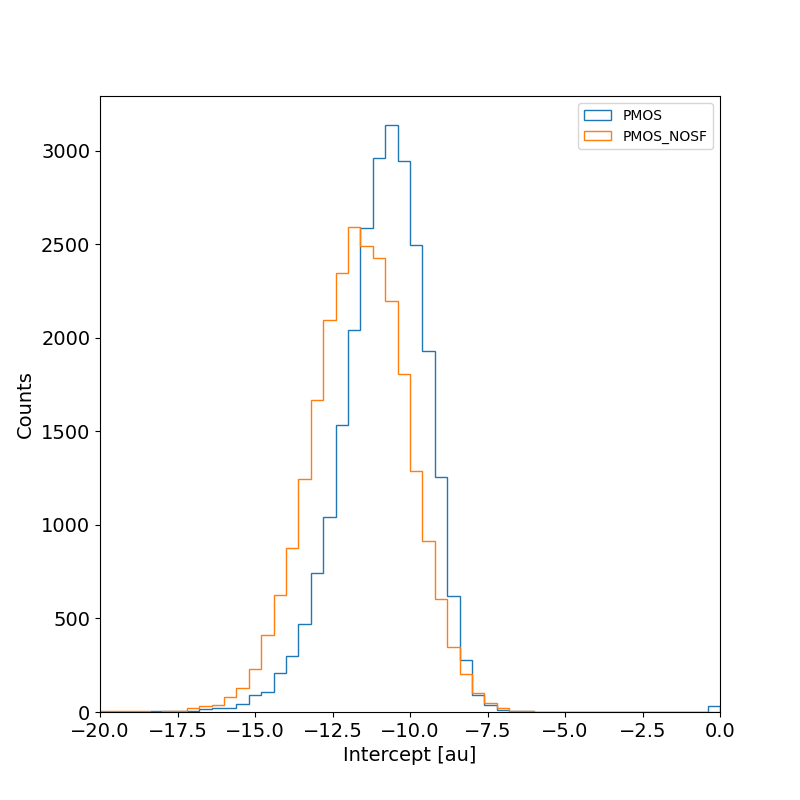
\includegraphics[width=.98\linewidth]{figures/charaterization/intercept_histogram.png}
            \caption{}
            \label{fig:}
            \end{subfigure}
        \end{figure} 

        \begin{figure}[h!]
            \begin{subfigure}{.5\textwidth}
            \centering
            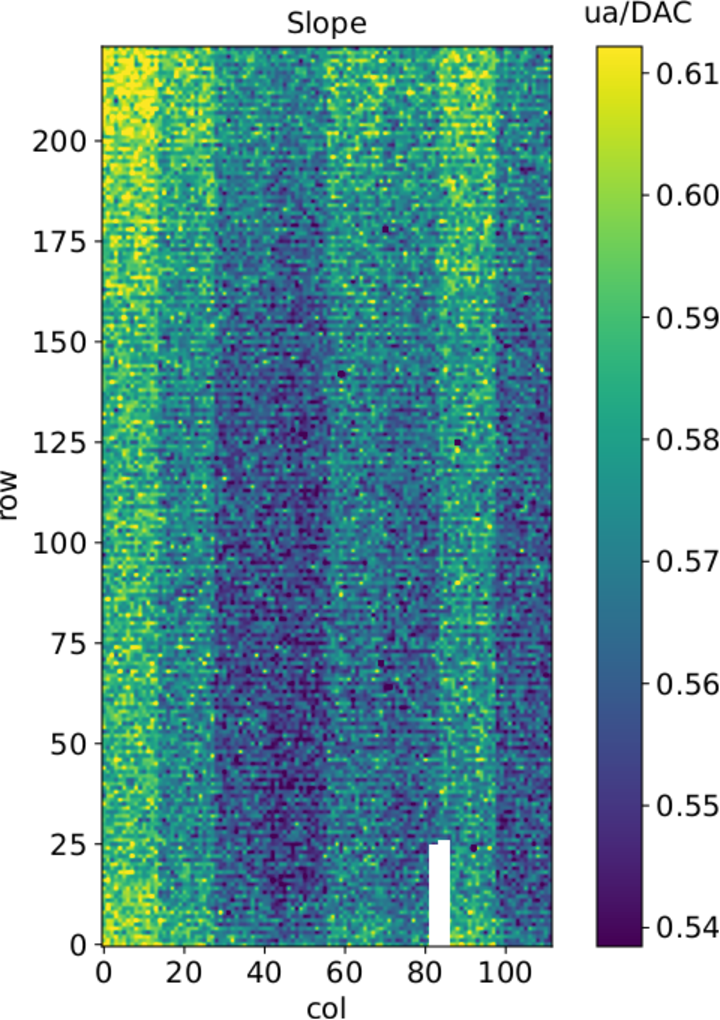
\includegraphics[width=.99\linewidth]{figures/charaterization/slope_map.pdf}
            \label{fig:}
            \end{subfigure}
            \begin{subfigure}{.5\textwidth}
            \centering
            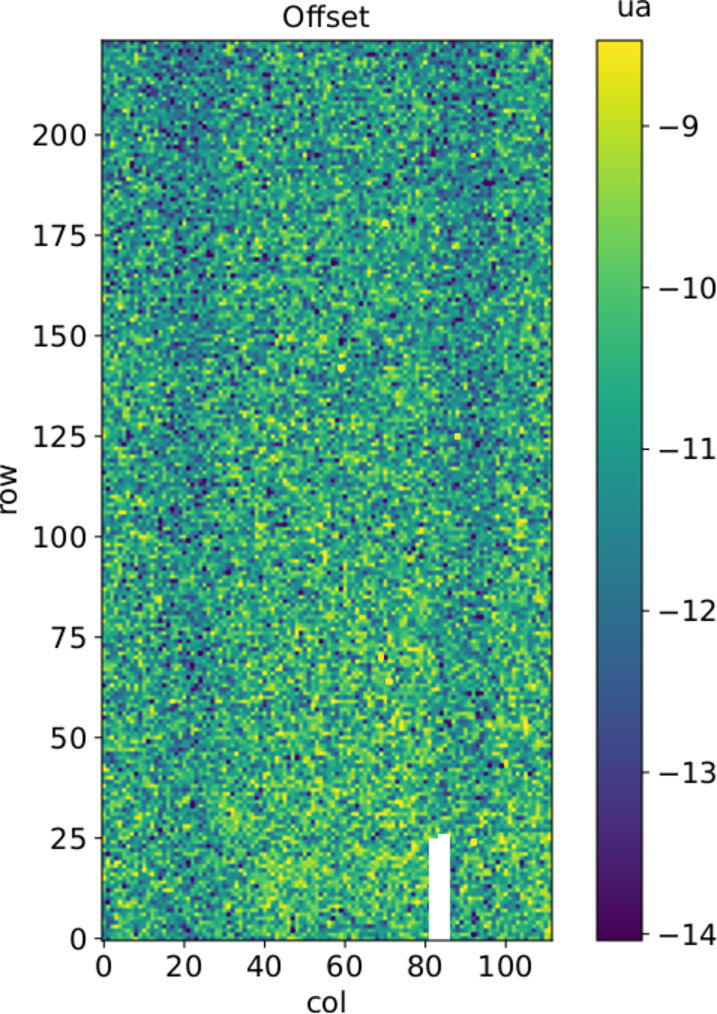
\includegraphics[width=.99\linewidth]{figures/charaterization/offset_map.pdf}
            \label{fig:}
            \end{subfigure}
            \caption{}
        \end{figure} 

        \begin{table}
            \begin{center}
            \begin{tabular}{| c |  c | c | c |c |}
            \hline
             & PMOS & & HV \\
            \hline
            \hline
            Slope [au/DAC] & 0.57145 $\pm$ 0.00025 \\
            Slope dispersion [au/DAC] &  0.01685 $\pm$ 0.00016\\
            Intercept [au] & -10.824 $\pm$ 0.019 \\
            Intercept dispersion [au] & 1.225 $\pm$ 0.013\\
            \hline
            \end{tabular}
            \caption{}
            \label{tab:}
            \end{center}
        \end{table}        

        \subsubsection{Absolute calibration}
        %python3 -i acquisition_Fe55/fit_tot_single_pixel.py -f acquisition_Fe55/source_PMOSS/Fe_acquisitions_6V/ per fare i fit. Attenzione che prende i file degli istogrammi npz già
        Per effettuare quest'utlima serve un segnale di cui si conosce il valroe in elettroni con una ragionevole precisione: per questo motivo la linea generata da un fotone da \SI{5.9}{keV} di dec del ferro 55 può risultare comoda. 
        Questo fotone viene assorbito nel silicio con una lamda di.. \\
        considerando uno spessore dello strato epitassiale svuotato di \SI{25}{\um} quindi la P di essere assorbito è: 
        Il fotone fa fotoelettrico ed emette un elettrone della stessa energia del fotone; ricordando che una particella carica produce mediamente una coppia electron-vacuum every \SI{3.65}{eV}, then the signal produced by the Fe55 source is expected to be \SI{1616}{e-}. 
        
        Il picco del ferro corrisponde agli eventi dove c'è assorbimento totale sul pixel e quindi dove vengono raccolti tutti i 1616 elettroni, mentre nella coda a sx del picco cadono tutti gli eventi con assorbimento parziale e/o incompleto dovuto anche a charge sharing.  
        Motivo per cui ad esempio in monopix due hanno fatto i pixel più piccoli: per ridurre la charge sharing riducendo così nel segnale la coda a sx. 
        Notiamo negli istogrammi alle figure \ref{fig:} e \ref{fig:} che tra i pixel ci può essere una visibile differenza tra quanto il picco sia pronunciato. In particolare questa differenza mosgtra che per le righe da 0-111 e 112-224 ..

        \red{Parla della differenza tra fit sopra e sotto nella amtrice}
        
        \begin{equation}
            f(x, N, \mu, \sigma) = \frac{N}{\sigma \sqrt{2\pi}} e^{-\frac{1}{2}(\frac{(x-\mu)}{\sigma})^2}
        \end{equation} 

        \begin{equation}
            f(x, m, q, N, \mu, \sigma) = m\,x + q + \frac{N}{\sigma \sqrt{2\pi}} e^{-\frac{1}{2}(\frac{(x-\mu)}{\sigma})^2}
        \end{equation}   
         
        \begin{figure}[h!]
            \begin{subfigure}{.5\textwidth}
            \centering
            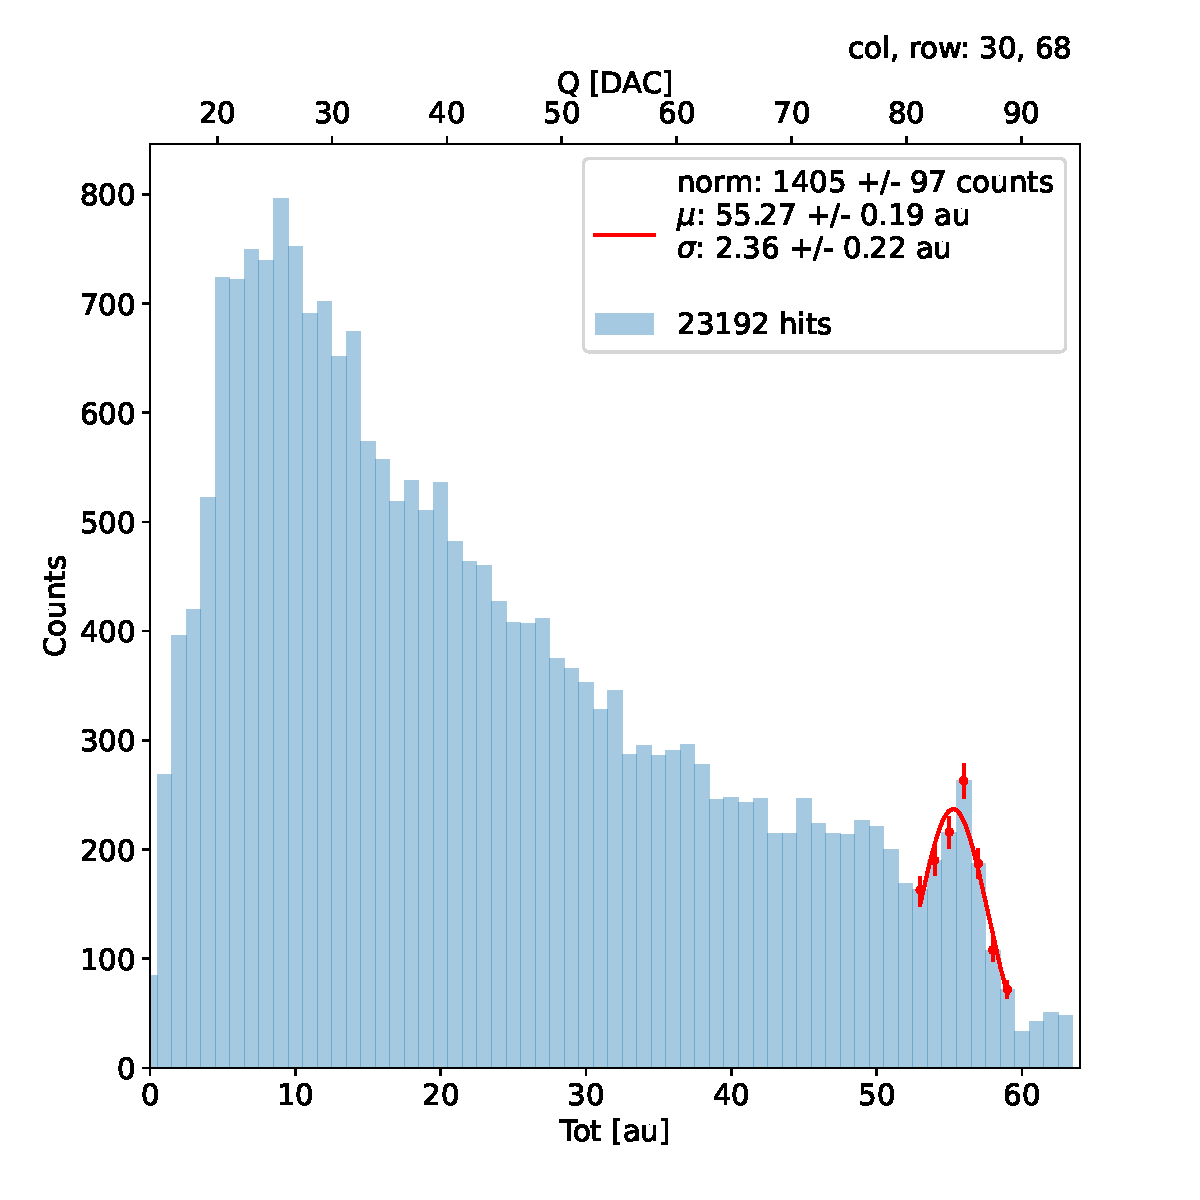
\includegraphics[width=.99\linewidth]{figures/charaterization/fit_gauss_r69.pdf}
            \label{fig:}
            \end{subfigure}
            \begin{subfigure}{.5\textwidth}
            \centering
            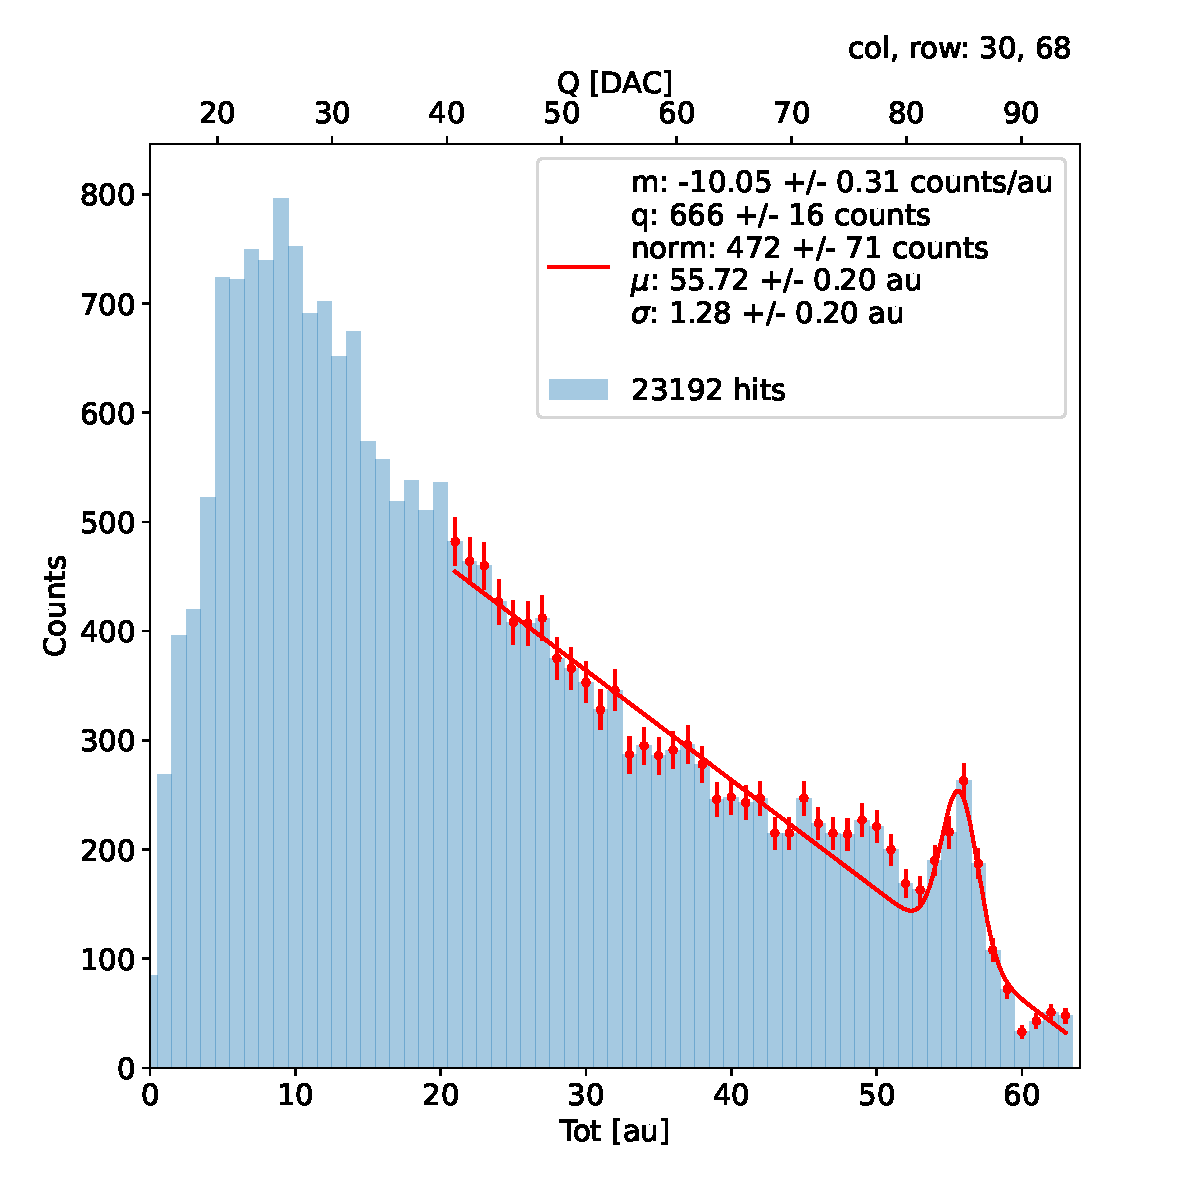
\includegraphics[width=.99\linewidth]{figures/charaterization/fit_line_gauss_r69.pdf}
            \label{fig:}
            \end{subfigure}
            \caption{due pixel per far vedere la differenza tra i fit}
        \end{figure}            

        \begin{figure}[h!]
            \begin{subfigure}{.5\textwidth}
            \centering
            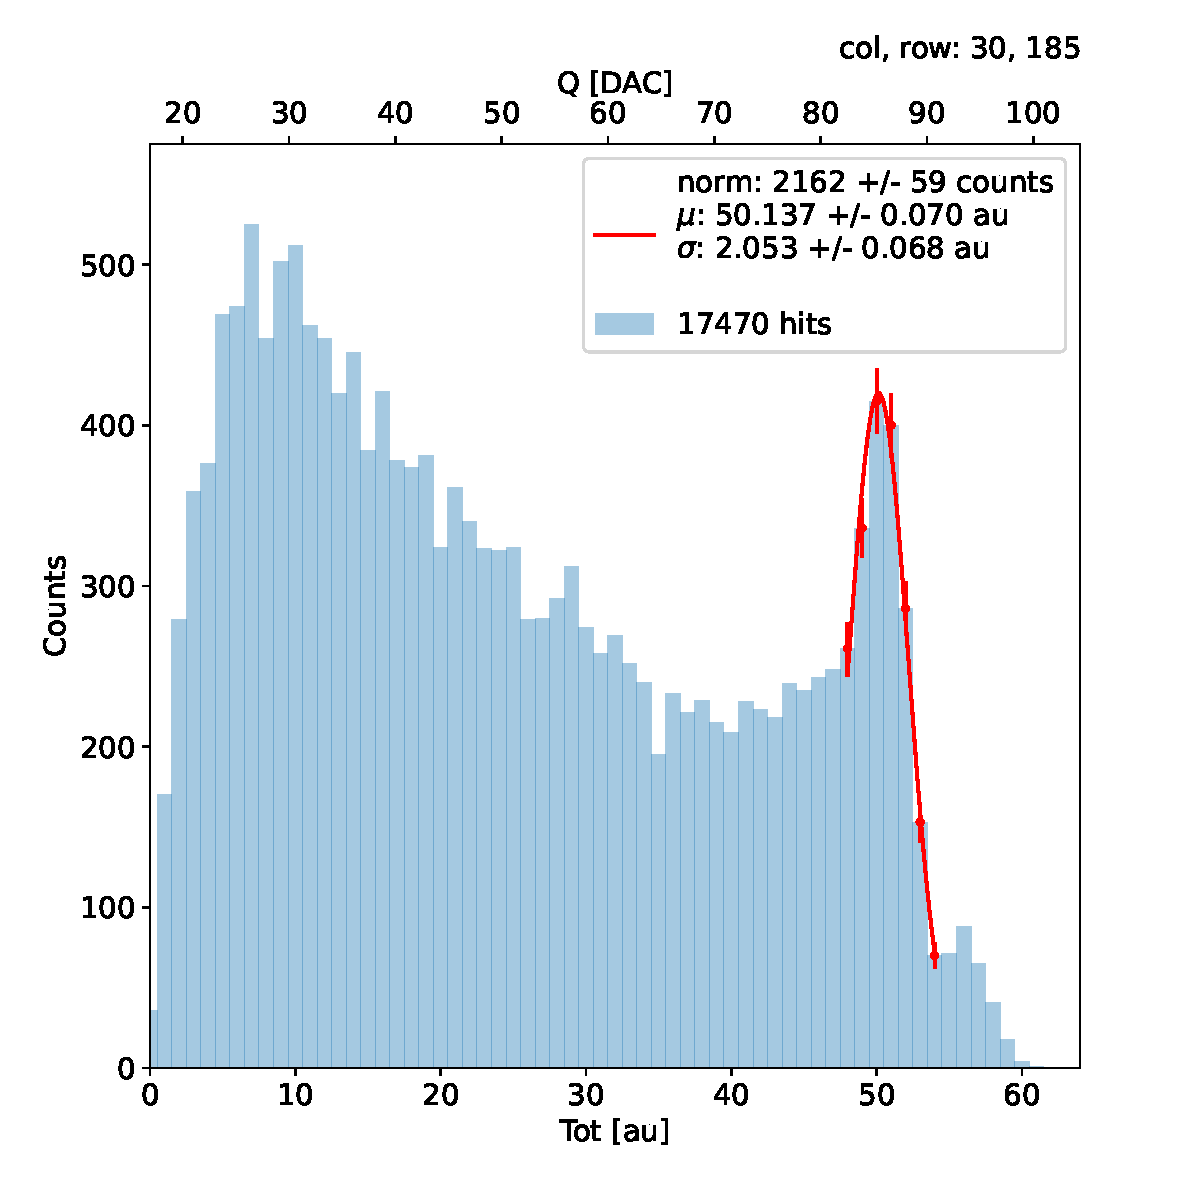
\includegraphics[width=.99\linewidth]{figures/charaterization/fit_gauss_r185.pdf}
            \label{fig:}
            \end{subfigure}
            \begin{subfigure}{.5\textwidth}
            \centering
            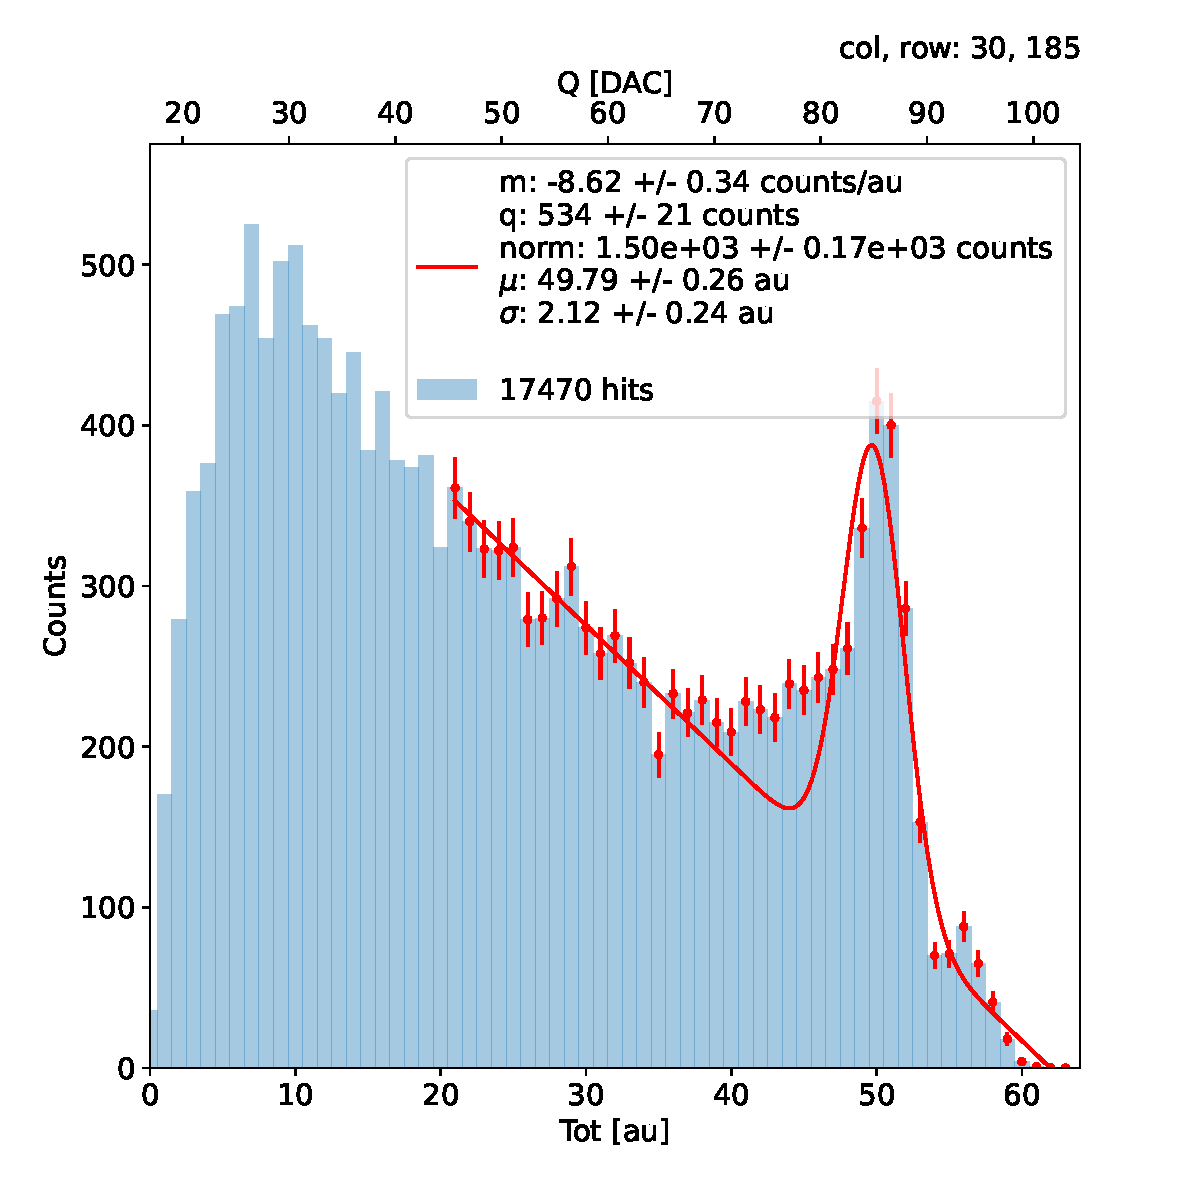
\includegraphics[width=.99\linewidth]{figures/charaterization/fit_line_gauss_r185.pdf}
            \label{fig:}
            \end{subfigure}
            \caption{due pixel per far vedere la differenza tra i fit}
        \end{figure}    

 
        
         \subsection{Fe vs bias}
         \begin{itemize}
             \item rate vs bias 
             \item posizione del picco del ferro vs bias    
             \item eventi sotto il picco vs eventi nella coda
         \end{itemize}
     
     
     \subsection{Measurements with radioactive sources}
         \red{CI metterei i plot con ferro, stronzio e cosmici}
         %python3 -i acquisition_Fe55/find_cluster.py -d acquisition_Fe55/source_PMOSS/noise_acquisitions_6V -> per cluster dimension e spettro del noise
         %python3 -i acquisition_Fe55/hit_map.py -f acquisition_Fe55/source_PMOSS/2022-04-07/2022-04-07_10-10-01_acq.h5 -> per le hit map, comprese qualche hitmap dei cluster
         %python3 -i acquisition_Fe55/Sr90_spectrum.py -d acquisition_Fe55/source_PMOSS/noise_acquisitions_6V/ -> per fare i plot dello stronzio
         ToT con doppia scala (calibrata in elettroni e non in ToT)
         hit per cluster
         dimensione cluster
         hit map di un paio di tracce?
        \subsection{Dead time measurements}
        The hit loss is due to analog and digital pile up: the first one occurs when a new hit arrives during the pre-amplifier response, the second instead, which is the more relevant contribution with high rate, while the information of the previous hit has not yet been transferred to the periphery.  
        As only one hit at a time can be stored on the pixel's RAM, until the data have completed the path to get out, the pixel is paralyzed and the dead time $\tau$ almost corresponds with the time needed to trasmit the data-packets off-chip.
        Since the exportation of data from pixel to the EoC occurs via a 21-bits data bus, only one clock cycle is need to transfer the data to the end of column and the dead time bottleneck is given by the bandwidth of the serializer at the EoC. In our setup the serializer operates at 40 MHz, thus to transmit a data packet (27-bit considering the addition at the EoC) at least \SI{675}{ns} are needed. 
        For what we have said so far, the R/O is completely sequential and therefore is expected a linear dependence of the reading time on the number of pixels to read:
        \begin{equation}
            \tau =\, 25\: \unit{ns}\, \times\, (\alpha\, N +\, \beta)
            \label{eq:reading_time}
        \end{equation}
        where $\alpha$ and $\beta$ are parameters dependent on the readout chain setting. 
        
        To measure and test the linearity of the reading time with the number of pixels firing, I have used the injection mode available on the chip. 
        Indeed, the injection mode allows fixing not only the amplitude of the pulse, which corresponds to the charge in DAC units, but also the period and the width.
        I have injected a fix number of pulses (100) and looked for the rate when the efficiency decreases. 
        Moreover to test that there is no dependece of the digital readout time from the charge of the pulse, I have try to change the amplitude of the pulse injected, but the parameters found were consistent with the default configuration ones.

        \red{Al posto degli esempi con 5 e 10 pixels metterei un esempio dell'efficienza vs il periodo quando leggo un singolo pixel. Una cosa che volevo fare era anche provare a fittare la slope con cui l'efficienza scende: se la slope è uguale per tutti il readout diventa completamente predittivo. }
        \begin{figure}[h!]
            \begin{subfigure}{.5\textwidth}
            \centering
            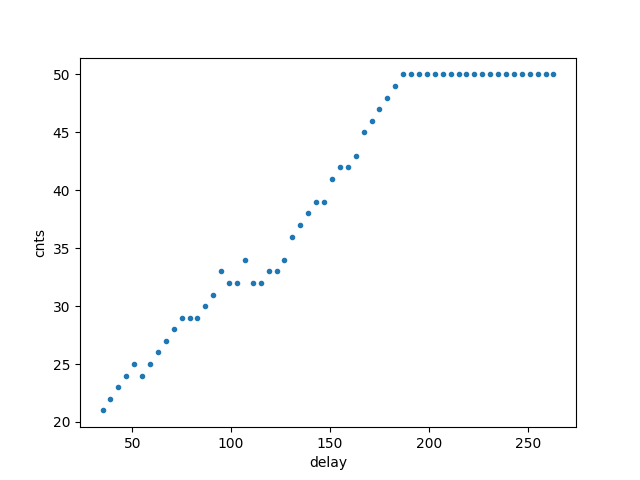
\includegraphics[width=.98\linewidth]{figures/charaterization/efficiency_5pixels.png}
            \caption{\red{efficiency vs DELAY 5 pixels}}
            \label{fig:}
            \end{subfigure}
            \begin{subfigure}{.5\textwidth}
            \centering
            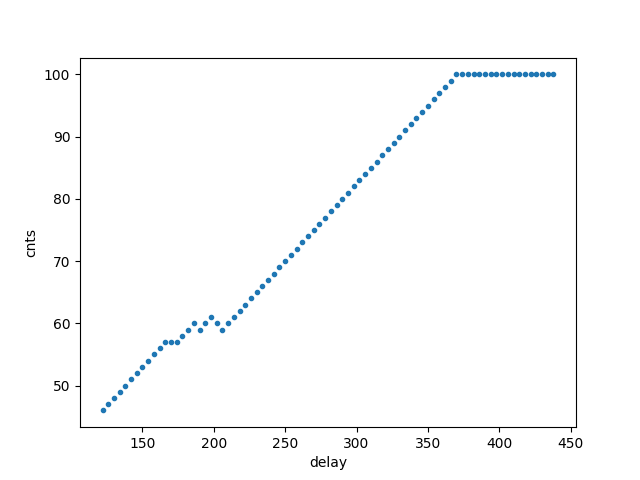
\includegraphics[width=.98\linewidth]{figures/charaterization/efficiency_10pixels.png}
            \caption{\red{efficiency vs DELAY per 10pixels}}
            \label{fig:}
            \end{subfigure}
        \end{figure}
        
        While the single pixel reading time and the dead time do not depend on the position on the pixel matrix and are equal to \red{106 (46+60)} clock counts within 1 clock count, on the other hand the $\tau$ depends on the pixel position on the matrix when more than one pixel are firing. 
        In particular the priority chain goes from row 224 to row 0, and from col 0 to 112, that means the last pixels to be read is the one on le bottom right corner of the matrix. 

        In figure \ref{fig:dead_time} is reported the reading time versus the number of pixels injected; the R/O parameters that control the reading time and their default values are reported on table \ref{tab:tab:R/O_param}.
        \begin{table}
            \begin{center}
            \begin{tabular}{|c | c | c |}
            \hline
            Parameter & Value [\si{DAC}] & Value [\si{\us}]\\
            \hline
            \hline
            START\_FREEZE & 64 & 1.6\\
            STOP\_FREEZE & 100 & 2.5\\
            START\_READ & 66 & 1.65\\
            STOP\_READ & 68 & 1.7\\
            \hline
            \end{tabular}
            \caption{Default configuation of the R/O parameters}
            \label{tab:R/O_param}
            \end{center}
        \end{table}

        The factor $\alpha$, referring to eq. \ref{eq:reading_time} is proportional to the difference (STOP\_FREEZE - START\_READ), while the offset $\beta$ lies between 5 and 15 clock counts.
        Since through the injection a random hit rate on the matrix can't be simulated, as the coordinates of the pixels to inject must be specified, for convenience I used the pixels on the same column/row. No difference in the $\alpha$ and $\beta$ coefficients has been observed between the two case. 
        \begin{figure}[h!]
            \centering
            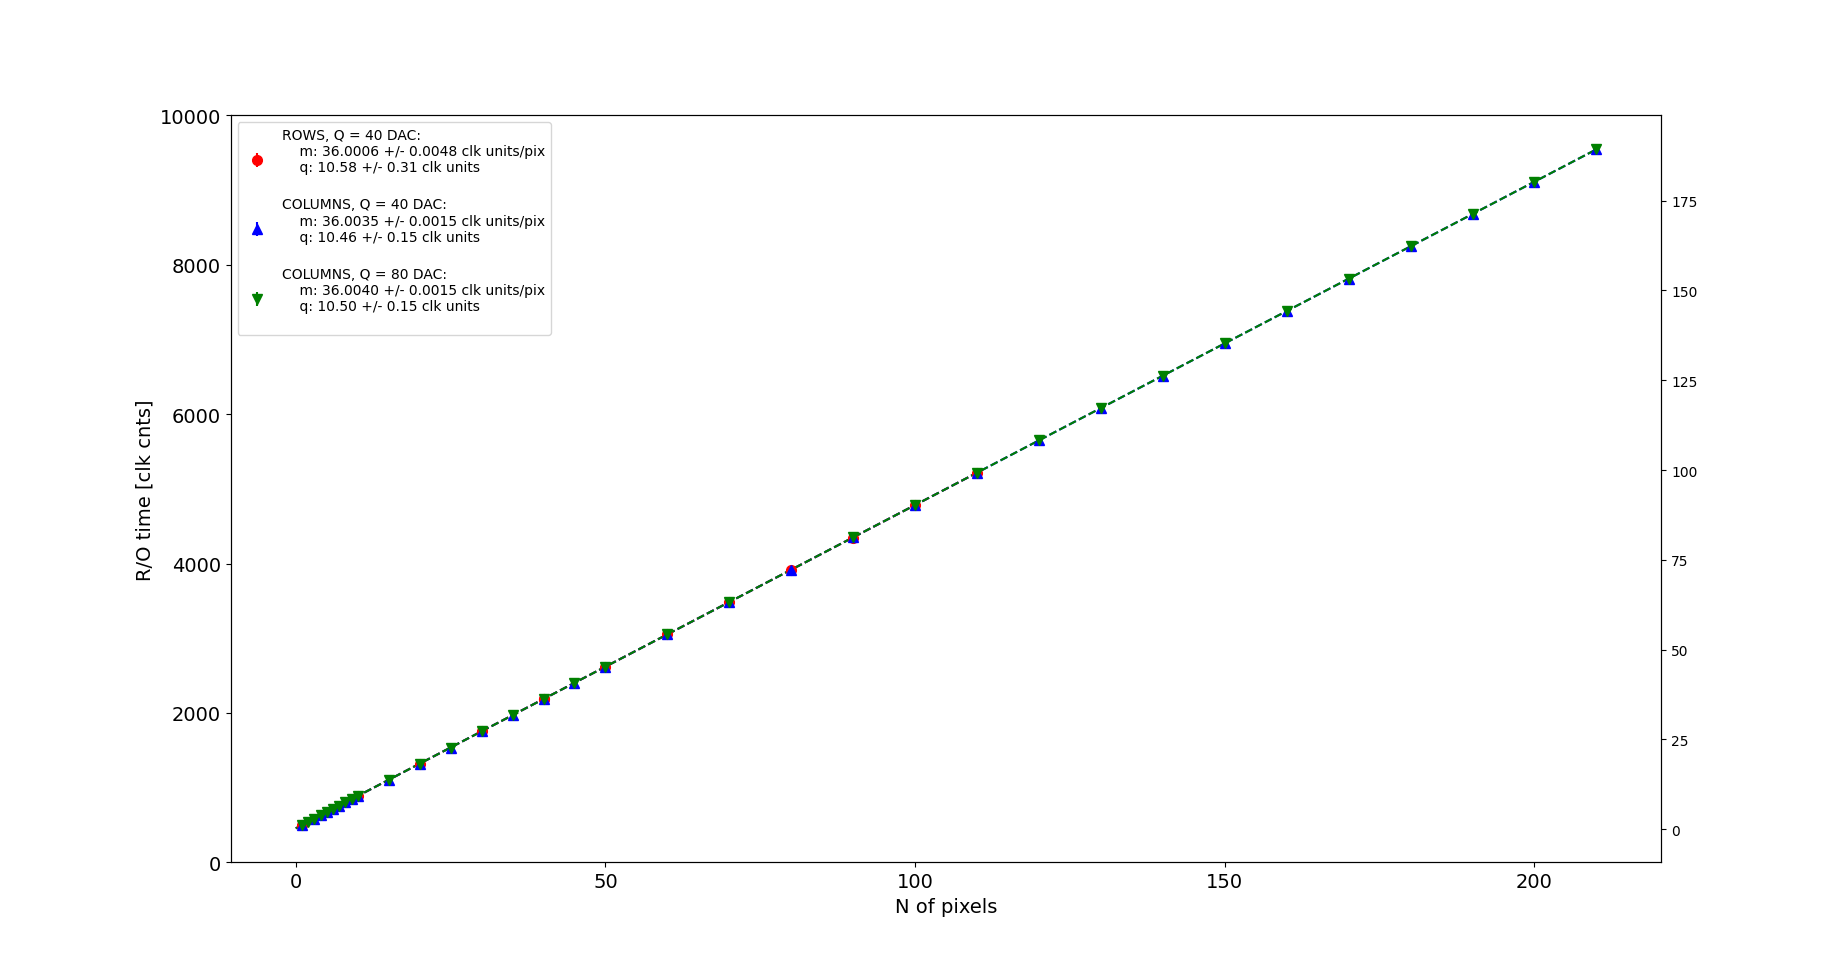
\includegraphics[width=.9\linewidth]{figures/charaterization/default_line.png}
            \caption{}
            \label{fig:dead_time}
        \end{figure}

        \begin{figure}[h!]
            \centering
            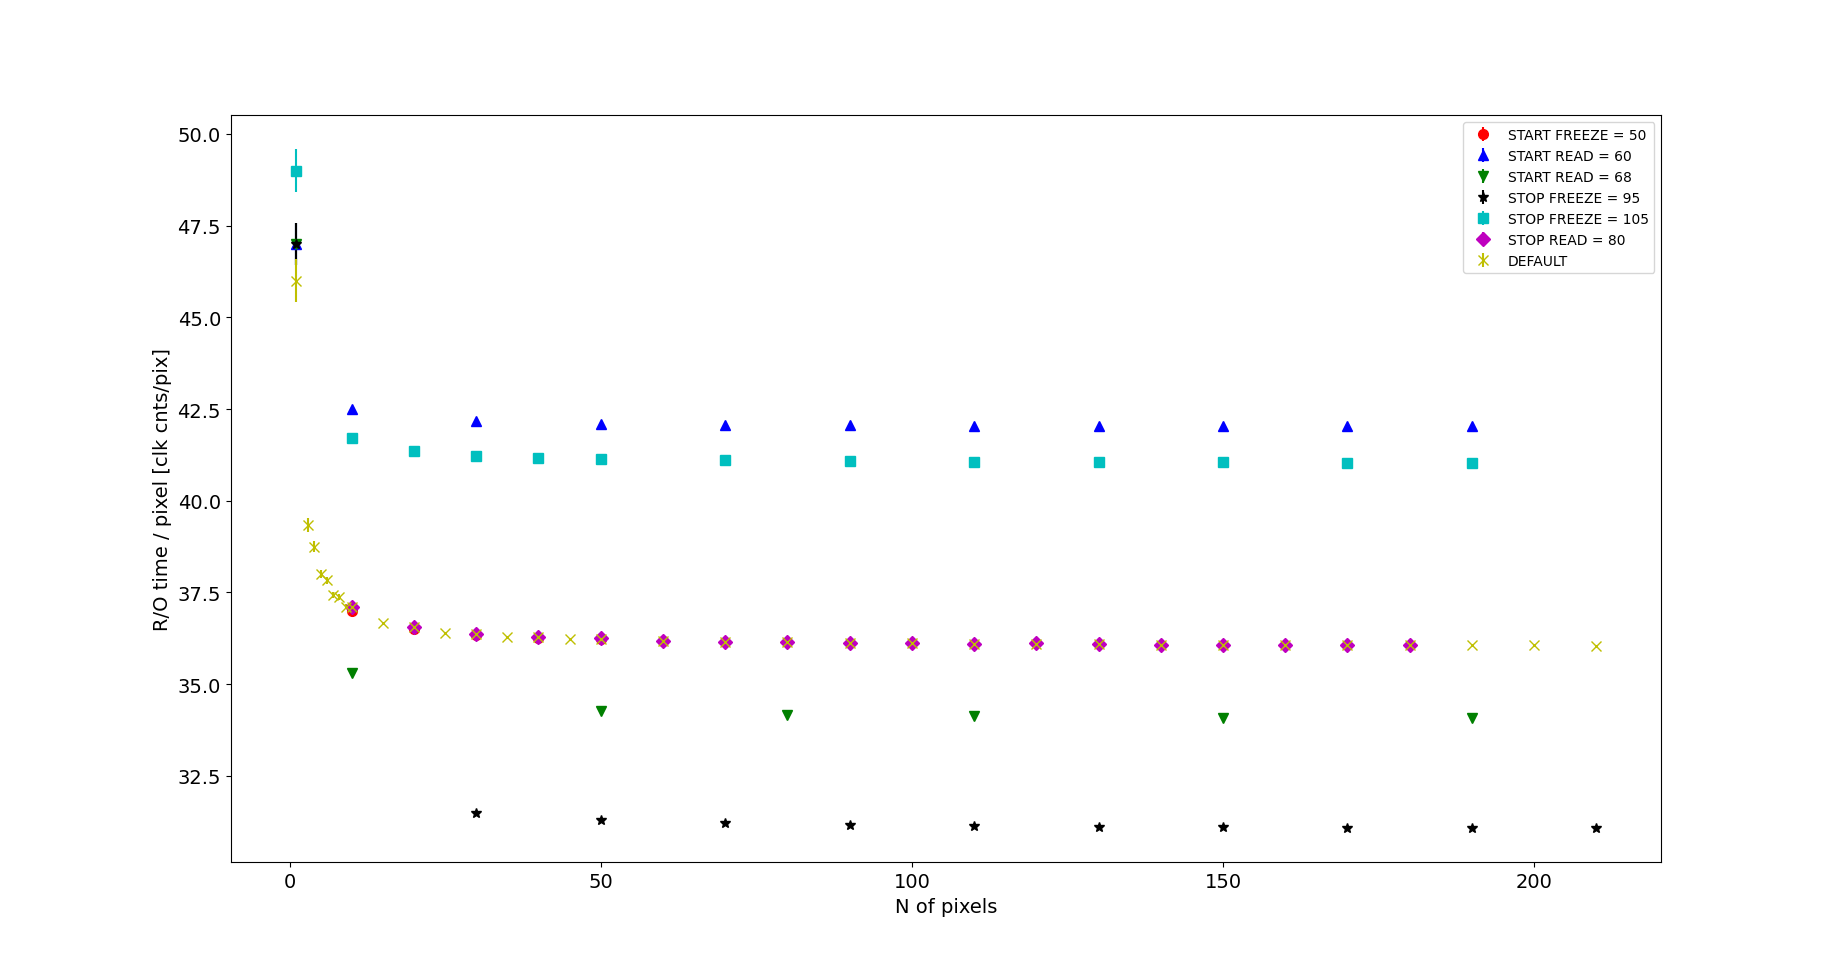
\includegraphics[width=.9\linewidth]{figures/charaterization/parameters_points.png}
            \caption{}
            \label{fig:dead_time}
        \end{figure}        

        \red{Ci sarebbe da spiegare perchè i parametri che usiamo noi come default non sono quelli che minimizzano il tempo di lettura. La spiegazione è che "Abbiamo copiato i valori dal repositorio di quelli di Bonn". Un'altra domanda potrebbe essere: come mai non ho esplorato una zona più vasta per i parametri del R/O. Cambiando molto i parametri del R/O la lettura non funzionava per niente: ad esempio CONF\_STOP\_FREEZE non può essere impostato nè sopra 105 nè sotto 95}



\section{ARCADIA-MD1 characterization}
